
\documentclass[12pt]{article}
\usepackage[english]{babel}
\usepackage[utf8x]{inputenc}
\usepackage{amsmath}
\usepackage{graphicx}
\usepackage[colorinlistoftodos]{todonotes}
\usepackage[margin=.8in]{geometry}
\usepackage{setspace}
\usepackage{multicol}
\setlength{\columnsep}{1cm}
\usepackage[
labelfont=sf,
hypcap=false,
format=hang,
width=.70\columnwidth
]{caption}
\usepackage{gensymb}

\begin{document}

\begin{titlepage}

\newcommand{\HRule}{\rule{\linewidth}{0.5mm}} % Defines a new command for the horizontal lines, change thickness here

\center % Center everything on the page
 
%----------------------------------------------------------------------------------------
%	HEADING SECTIONS
%----------------------------------------------------------------------------------------

\textsc{\Large Stanford Pozzuoli}\\[0.5cm] % Major heading such as course name
\textsc{\large The Roman Harbor of Puteoli}\\[0.5cm] % Minor heading such as course title

%----------------------------------------------------------------------------------------
%	TITLE SECTION
%----------------------------------------------------------------------------------------

\HRule \\[0.4cm]
{ \huge \bfseries Roman Concrete: Stressor Analysis in the Bay of Naples}\\[0.4cm] % Title of your document
\HRule \\[1.5cm]
 
%----------------------------------------------------------------------------------------
%	AUTHOR SECTION
%----------------------------------------------------------------------------------------

\begin{minipage}{0.4\textwidth}
\begin{flushleft} \large
\emph{Authors:}\\
Litawn \textsc{Gan}

Jake \textsc{Gold} 

Sierra \textsc{Killian}
\end{flushleft}
\end{minipage}
~
\begin{minipage}{0.4\textwidth}
\begin{flushright} \large
\emph{Professor:} \\
Dr. Tiziana \textsc{Vanorio} 
\end{flushright}
\end{minipage}\\[.75cm]

\begin{abstract}
We assess the durability of ancient Roman concrete and modern concrete with Portland cement in the marine environment of the Bay of Naples. The concretes are analyzed in the presence of stressors ranging from temperature, chemical interactions, and biomodification. We emphasize an interdisciplinary perspective throughout the analysis, and use physics, chemistry, and biology techniques. Ancient Roman concrete is found to be more resilient to almost all physical and chemical factors with the exception of wind. Its low permeability, reactivity, and thermal conductivity make the concrete an ideal base for marine structures and buildings. Modern concrete, though stronger than Roman concrete in terms of loads bearing capabilities, quickly reacts to marine stressors and deteriorates rapidly. We conclude that the integration of traditional Roman pozzolana recipes with modern manufacturing and reinforcement methods would lead to the ideal marine building material. Durability, strength, and longevity are crucial advantages of Roman concrete in the construction and development of coastal communities. 

\end{abstract}


\includegraphics[scale = .15]{Stanford_University_seal_2003_svg.png}\\[1cm] % Include a department/university logo - this 
\vfill % Fill the rest of the page with whitespace

\end{titlepage}

\onehalfspace
\twocolumn

\section*{Introduction}
\subsubsection*{Preserving the Ancient World}
The preservation of the ancient world is fundamental for mankind’s understanding of the past. Whether through archaeological evidence, scriptures, or cultural influence, historic civilizations are fundamental to our modern ideas and technologies. Natural weathering agents pose a major threat to the traces of ancient civilizations left on Earth, particularly in the marine environment. Submerged ruins experience the physical weathering of the surrounding water column, the chemical degradation from sea water contact, and deterioration from micro and macroorganisms. Understanding how these stressors act on ancient ruins is crucial in establishing effective conservation initiatives to preserve and restore the monuments of our past.

The Bay of Naples is an especially valuable cultural region, filled with historical landmarks and ancient ruins from the Roman Empire. Because the bay is a coastal environment by the Mediterranean Sea, ancient ruins face all the challenging stressors of the marine environment. 

\subsubsection*{Roman Concrete}

The primary construction material of ancient Roman ruins in the Bay of Naples is Roman concrete. The invention of concrete revolutionized the Roman empire and spurred the creation of some of the most well known archaeological ruins today. The date of its invention is unknown; it was introduced in the late Roman Republic, and saw widespread use throughout the lifetime of the Roman Empire. The uncommon strength and durability of the material inspired the Roman Architectural Revolution, a cultural shift in construction from solely functional purposes to artistic and aesthetic motivations. Liberated from utilitarian shape, previously rare forms like the arch, dome, and vault became popular throughout the empire.

Our knowledge of the recipe for Roman concrete (RC) is limited, however, the writings of Vitruvius suggest that RC is a mixture of hydraulic cement made with lime and pozzolana and aggregates of brick, ceramic, or rocks. The Romans used volcanic ash within the region surrounding Naples for the pozzolana component. When exposed to water and the calcium hydroxide in lime, the aluminosilicates form calcium silicate hydrates, making the mixture cementitious with high aluminum and silica content.

\subsubsection*{Modern Concrete}
    
Modern concrete (MC) is formulated with Portland cement and aggregates such as rock or sand. The material has become ubiquitous in the modern world, as engineers exploit its durability, availability, and economic advantages to construct structures all over the globe
. Like RC, MC consists of a hydraulic cement rich in calcium silicates that hardens in the presence of water. MC differentiates from RC in the use of modern manufacturing techniques and metal reinforcement. 

\subsubsection*{Comparing Concretes}

As concretes with hydraulic cements, both MC and RC can be set and hardened in marine environments. This property has proved crucial for RC: the Bay of Naple's tectonic activity has led to bradyseism and periods of uplift and subsidence, and Roman constructions have been submerged beneath the Mediterranean for years. Ancient remnants of harbors, houses, and cities are still being uncovered in the Bay of Naples today, despite exposure to marine stressors. This longevity is indicative of RC's strength and durability in marine environments.

In contrast, MC has not been tested as extensively as RC. Their difference can be inferred by analyzing the effect of adding pozzolana into the MC recipe to approximate RC. Adding pozzolana alters fundamental properties of the material that change its response to stressors. While a large body of research exists with analysis on the deterioration of concrete with respect to specific stressors, we incorporate physical, chemical, and biological stressors in the marine environment to produce a cogent analysis of the entire degradation process.

\section*{Physical Factors}

The preservation of concrete structures within the marine environment is largely determined by its resistance to a fluids. Periodic exposure to vector forcings, atmospheric conditions, and daily temperature variations can exaggerate marine concrete degradation. Physical stressors include: hydrostatic load, waves, tides, winds and temperature.

\subsection*{Fluid Stressors}

\subsubsection*{Hydrostatic Load}

Hydrostatic load is defined as the total force exerted by the surrounding water column on a region of concrete (Banthia, 2001). The compressive force is exerted radially, increasing by one atmosphere for every 10 meters of depth (Sverdrup, 2007). Depending on the permeability of the concrete, hydrostatic load may distribute itself both on the outer structure and within. Hydrostatic load does not change significantly on a submerged structure in a small timescale: wave action and tides add little to depth variation. The result is a constant exertion of water pressure on the structure. 

However, for concrete exposed to both wave and tidal action as well as winds, the hydrostatic load fluctuates. During desiccation periods (low tides or warmer days) the water within the concrete begins to expand and exert a larger force on the internal structure. This can lead to cracking which weakens the overall load bearing capabilities of the concrete (Banthia, 2001). Cracking refers to shattered or separated segments in cement that releases their load to the surrounding concrete. Cracks form near or around deteriorated fibers in the cement due to the increased stress released after the fibers fail (Hasson, 1988). Generally, RC cracks laterally with respect to the banded cement strata between aggregate layers. The aggregates forms a band that resistant vertical cracks (Vanorio, verbal communication). MC on the other hand can crack both laterally, vertically, and radially depending on the aggregates used and the internal support fibers. The variation in directionality allows for an increased chance of cracks connecting and then spalding. 

\begin{figure*}[ht]
  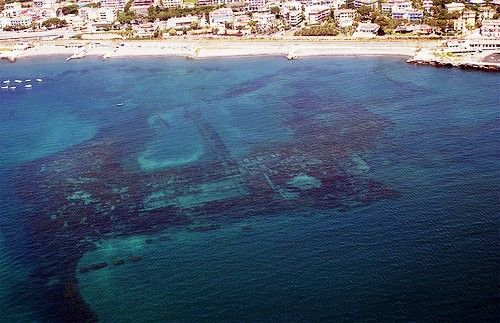
\includegraphics[width=\textwidth,height=12cm]{port_julius.jpg}
  \caption{Submerged Port of Julius in the Bay of Naples, primarily made of Roman concrete and brick work. Photography by Sherry Tomaselli.}
\end{figure*}

\subsubsection*{Waves and Tides}

In addition to the forcing of water on concrete, waves and tides add fluctuating stress vectors to both RC and MC. Though the Mediterranean Sea is an isolated body of water, the large surface area allows for the formation of both wind driven waves and tidal cycling. The Pozzuoli region is 41 degrees north latitude and experiences a semi-diurnal tidal cycle, with two daily high and low tides. The tidal range within the Naples inlet has a magnitude of 3-5 cm. In comparison to the large size of the concrete structures, 3-5 cm variation in tidal range does not result in high exposure and submergence. 

Long term sea level change is much more important. Since the bay of Naples is constantly subsiding and uplifting because of bradyseism, different parts of the concrete will be exposed in the long run. Those regions closer to sea level or the splash zone will experience a faster rate of degradation than submerged or dry regions. The 0.25-1.0 foot waves on the other hand are both a short term and long term issue. Periodic exposure during the troughs of the waves followed by a high hydrostatic forces during the waves’ crests forces the concrete in and out of a compressive state. These fluctuations drastically increase the compressive and tensile forces acting on the concrete. 

Between RC and MC, RC is more resistant to long term exposure to hydrostatic forces. The lower permeability prevents refilling of cracks and pores on a regular basis. Overtime, the MC is more likely to experience cracking and deterioration due to periodic exposure to dry and wet conditions (Hasson, 1988). However, both cements hold up equally well when completely submerged. MC, being a stronger concrete than RC may handle the hydrostatic load better overtime. However, engineers need to consider other factors as well, as MC is generally weakened faster than RC due to other physical and chemical factors. 

\subsection*{Wind Erosion}

Wind erosion, while weaker than waves and tides, is a significant stressor for exposed concretes. Structures built within the intertidal or supratidal zone, as well as the subtidal zone if tall enough, experience extra forcing from wind stress (Sverdrup, 2007). The wind applies both a compressive and tensile force. Internal fibers such as steel bars in MC help distribute the load of wind stress. Winds also carry particulate matter that can strike the concrete structure causing long term degradation through low angle and direct impacts. 

Low angle particulate collisions scratch the outer layer of concrete, scraping away cements and aggregates and reducing structural integrity. Over time, the accumulation of scratches erodes the outer concrete layers, exposing the internal layers to a variety of new physical and chemical stressors. 

A direct impact, on the other hand, causes indentation and fracturing. The compressive strength of impacting particles forms micro-cracks and fractures the concrete over time. Though it doesn't necessarily strip away the outer layers, direct impact exposes new surface area to physical and chemical stressors by cracking (Yunhong, 2016). Both RC and MC fare equally well against wind erosion, as adding pozzolana doe not increase resistance. However, as RC is a more resistant concrete to chemical weathering, the long term surface area exposure caused by cracking and scratching will be less detrimental than in MC (R.K, 2014). All stressors work additively, and their correlations remain significant. 

\subsection*{Thermal Conductivity}

In comparison to other types of materials, concrete of all types is characterized by low thermal conductivity, contributing to their popularity in construction. The International Standard for building materials and products lists the thermal conductivity of concrete, $k$, as anywhere from 1.65 to 2 watts per meter per Kelvin $(W*m^{-1}*K^{-1})$ without metal reinforcement (ISO, 2007). In comparison, aluminum has a thermal conductivity of about 205 $W*m^{-1}*K^{-1}$.

A more thorough analysis of the thermal properties of concrete reveals nuances. Consisting of aggregate combined with mortar paste, both RC and MC can be considered two-phase materials with complex interactions between the two components. The exact equation for this behavior is contested; a proposed formula appears in Campbell-Allen and Thorne treatise (D. Campbell-Allen, 1963):
$$k = k_m (2M-M^2)\frac{k_m k_g (1-M)^2}{k_g M + k_m (1-M)}$$
$$M = 1 - (1-p)^{1/3}$$
where $k_m$ and $k_g$ are the thermal conductivity of mortar and coarse aggregate, respectively, and $p$ is the volume of mortar per unit volume in concrete.  Of note: empirical tests of the prediction model report increased inaccuracy with high aggregate conductivities. In addition, humidity, fine aggregates, and concrete age were not encompassed by the model despite non-negligible interactions with thermal conductivity. The equation is nevertheless widely cited in concrete literature and is a valuable heuristic tool for determining thermal behavior.

According to the equation, the conductivity of the consolidated concrete depends on ${k_m}^2$ and $k_g$. Pozzolanic ash in roman concrete, added to the mortar, would have contributed to the more sensitive $k_m$ term. No conclusive thermal conductivity prediction model for Roman concrete exists; however, research on incorporating fly ash, a pozzolanic material, in concrete unambiguously reduces $k$. This behavior has been attributed to heat of hydration, a chemical consequence of using pozzolanic concrete (Bessenouci, 2011).

Lower thermal conductivity in pozzolanic-based concrete indicates that RC has more thermal resistance to heat loads than MC. This difference in thermal conductivity is the basis for comparing the behavior of RC and MC in high temperature/low temperature environments. MC will be more susceptible to temperature fluctuations than RC. 

\subsubsection*{Land-locked Concrete}

Land-locked concrete is very resistant to extreme temperatures, with no deterioration from temperatures of 0$\degree$C to 300$\degree$C. Water caught in pores freezes below 0$\degree$C, expanding in volume by about 9\% and straining the concrete. Above 300$\degree$C, the aggregate continues to expand while the mortar contracts due to water loss, compromising the integrity of the material (Portland, 2002).

\subsubsection*{Marine Concrete}

Concretes in marine environments, on the other hand, are incredibly sensitive to temperature. Heat can be a driving force of deterioration, as it accelerates the rate of chemical and electrochemical reactions that aggravate the concrete. A heuristic rule derived from the classical law (the Arrhenius equation) suggests that for each increase of ten degrees Celsius in temperature, the rate of chemical reaction approximately doubles (Mehta, 1990).  The exact relationship is dependent on activation energy and other factors; however, increasing temperatures will almost always accelerate chemical reactions. Because of this correlation, temperature is significant factor in marine concrete decay.

The average temperature in central Italy is about 17.5-19$\degree$C, with local and seasonal variations throughout the year. Ocean temperatures fluctuate by about 6$\degree$C throughout the day, so any discrepancy in thermal conductivity is relevant between RC and MC. With this in mind, we can expect RC to fare better than MC against heat-induced degradation in a marine environment.


\section*{Chemical Factors}

Chemical degradation mechanisms are significant in concrete, especially in the marine environment, where ions can attack concrete from seawater and air. For the Bay of Naples, the Mediterranean Sea is an effectively infinite source of reactive elements like salt, chloride, and carbon dioxide. To exacerbate the situation, water is constantly flowing and recharging the reactive elements. Chemical factors include: carbonation, sulfates, ionic interactions, alkalinity, and salt.

\subsection*{Carbonation}

The most common type of reaction for any concrete is carbonation (Winter, 2005). The Bay of Naples is one of the most active geothermal sites in the world, and carbon dioxide is constantly outgassed by fumerals both on land and underwater. Higher levels of carbon dioxide in seawater lead to the formation of carbonic acid (HCO3-) which dissociates to bicarbonate (H2CO3). The dissociation releases hydrogen ions into the water, lowering the overall pH. The ocean is naturally alkaline at a pH of 8.14, but the Mediterranean is more acidic at a pH of 7.95 (Luchetta, 2010).

Whether on land or underwater, structures are always exposed to carbon dioxide. The CO2 reacts with calcium hydroxide in the cement to form calcite (aragonite in hotter conditions). This is not necessarily harmful; the accumulation of calcite can increase tensile strength and compressibility, strengthening the concrete (Winter, 2005). Depending on the porosity of the concrete, carbon dioxide rich water slowly seeps into successively deeper layers, creating dissolved calcites. The reaction occurs much slower in RC than in MC due to its lower permeability. If MC is reinforced with steel, the process of carbonation and exposure to carbon dioxide can rapidly corrode the beams. This causes expansion and a weakening of the overall structure (Vanorio, verbal communication). The rusting beams can expand enough to remove large pieces of concrete, termed spalding. 

\subsection*{Sulfates}

Sulfates are highly reactive with external carbon groups in the concrete. The reaction produces gypsum, then forms ettringite which eventually dissociates to monosulfate. The loss of external carbon groups due to sulfate attacks gradually degrades the external layers of concrete. Since MC is much more permeable than RC, sulfate attacks can also occur internally. In this scenario, the formation of ettringite pushes the surrounding concrete; causing cracking and expansion. Overtime, the MC cement and aggregate may become separated from one another; severely reducing the load of the structure (Astier, 2014). RC doesn’t readily experience internal sulfate attacks because water cannot enter internal cavities. The result is a more durable concrete structure that lasts longer than MC with respet to sulfate decay (R.K, 2014).



%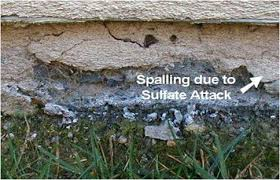
\includegraphics[width=8cm,height=6cm]{spalling.jpg}
%\captionof{figure}{Concrete decay induced by spalling and cracking. From the International Journal of Emerging Trends in Engineering and Development.}

\subsection*{Salt Attacks}
    
Salt attacks pose similar issues to concrete as sulfate attacks. The reactivity of chloride ions with external CH groups weakens the structural integrity of the concrete (Neville, 1995). The formation of ettringite is also a problem with chloride ions, especially in the Mediterranean Sea which has an average salinity greater than 38 ppt (ocean is 35). Salt attacks are particularly destructive in the subtidal and supratidal zones around coastal areas. The periodical exposure to air and sea spray allows for the formation of mineralized salt crystals. As the concrete dries or is heated in the sun, the salt is left behind and begins to adhere to each other, forming halite deposits.


Much like the ettringite deposits, the salts exerts additional forces on the surrounding concretes and can cause loss of structural integrity. Another issue is the deterioration of the reinforcement in more modern concretes. Steel rebar is susceptible to oxidation and expansion when exposed to chlorides and sulfates (Kofi, 2014). Though MC does not usually use steel reinforcement in marine environments and is generally impermeable enough to prevent ionic intrusions, eventually any rebar used will rust and expand. This causes massive cracking and the removal of external pieces of concrete. RC does not have metallic reinforcement and is therefore more resistant to long term destruction. It less permeable than MC and resists most forms of ionic attacks (R.K, 2014).


The chemical difference between the two concretes convey distinct advantages in the marine environment. RC relies on its inert nature and impermeable structure to resist ionic attacks whereas MC is made with extremely low concentration of ions. The low initial ionic content in MC in combination with its stronger integrity makes it the ideal concrete for short term, heavy load bearing projects. However, in the long run, MC will saturate with ions and deteriorate, whereas RC will not (R.K, 2014).

\subsection*{Alkaline Degradation}

Alkaline attacks are a different form of concrete deterioration. Also known as concrete cancer, alkaline degradation is a chemical reaction where the alkaline nature of the cement reacts with the silica in the aggregate. This leads to expansion of the concrete by the formation of calcium silicate gel. Over time, alkaline attacks cause cracking and eventually spalding. Calcium hydroxide (Ca(OH)2) in the cement reacts with the silicic acid (H4SiO4) in the aggregate, creating the gel. As more Ca 2+ ions react, the gel pressures force expansion and weaken the concrete.

Once again, MC and RC have different resistive natures. MC is made with reduced alkaline cement; slowing the formation of calcium-silicate gels (Hasson, 1988). However, water cycled through the pores reacts to become alkaline, gradually allowing for alkaline attacks. RC is more alkaline to begin with, but has a lower pH pore fluid structure. This means the internal alkalinity remains low due to less reactivity of the surrounding cement with the water. MC is once again better in the short run, but over time RC reacts less and resists spalding by alkaline attacks. 

\begin{figure*}[ht]
  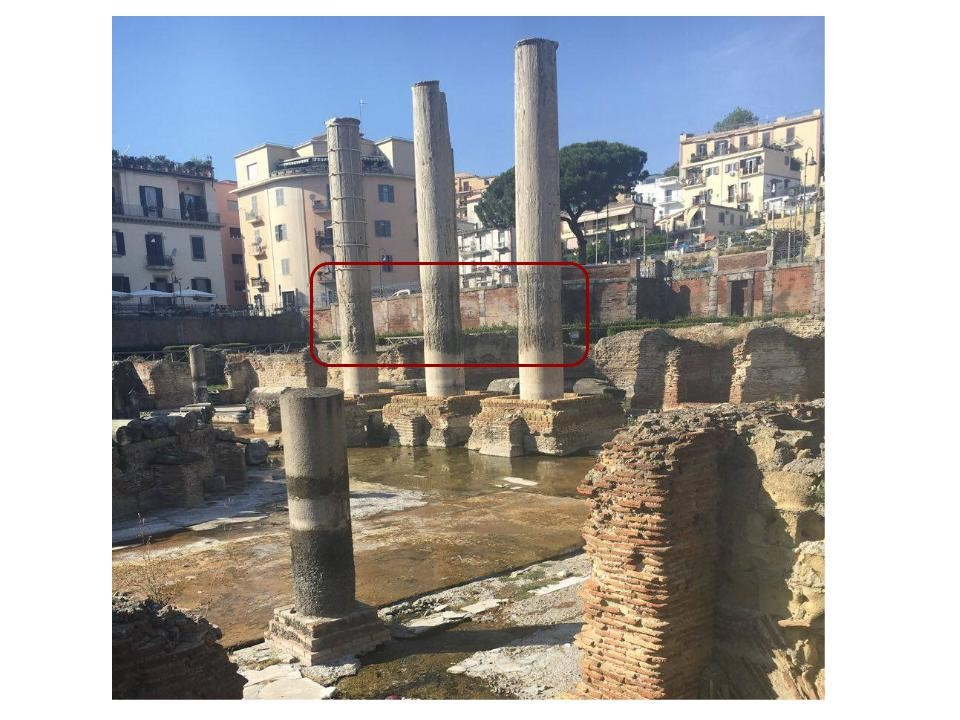
\includegraphics[width=\textwidth,height=12cm]{Bivalve_boreholes}
  \caption{Bivalve boreholes on the lower halves of the three central columns of the Macellum in Pozzuoli, shown in red rectangle.}
\end{figure*}

\section*{Biotic Factors}

In the Bay of Naples and throughout what was once the Roman empire, one of the largest threats to submerged ancient ruins is the biological activity of the Mediterranean.  Both large organisms, such as molluscs, and microorganisms, like fungi and algae, can contribute to deterioration.   
\subsection*{Macroorganisms}

The most obvious signs of biogenic deterioration to the naked eye are boreholes, generally found in calcareous artifacts.  The marble columns of Pozzuoli’s columns, for instance, are riddled with holes made by Lithophaga marine bivalves, as shown in figure 1, and studied by Morhange et al.  Lithophaga species bore holes into stone by secreting neutral calcium-binding mucoproteins, which dissolve the substrate (Jaccarini et al 1968).

An experiment with artificially placed limestone panels in nearby Baiae found that Rocellaria dubia, another bivalve species, began colonizing within a year of the installation of the panels (Casoli et al 2016).  Like Lithophaga bivalves, R. dubia use chemical secretions to bore holes; however, the species also use their shells for mechanical abrasion (Morton et al 2011).  Along with Lithophaga sp., R. dubia is one of the most important boring bivalves in the Mediterranean, and its effects on modern and Miocene submerged materials have been well-documented.  R. dubia boreholes significantly damaged the panels in Baiae, with some shells reaching 13 millimeters in length, the full thickness of the panel, after three years.  While similar studies have not been conducted with concrete as the substrate, the intensity and speed with which molluscan species can bore into calcareous material suggest that the underlying structure of many Roman remains may also be at risk from boring organisms.  Because modern construction uses calcareous rocks as its aggregate instead of the volcanic Neapolitan yellow tuff that the ancient Roman used, modern concrete is more susceptible to attacks by bivalves.

	The threat posed by endolithic marine macroorganisms, while significant, can be mitigated by changing several factors.  Most influential of these is sediment coverage. In the Gulf of Pozzuoli, ancient artifacts completely covered with sediment did not have any signs of biodeterioration, while exposed statues were severely damaged.  The statue of Ulysses found in the gulf shows the difference in bioerosion quite dramatically. From the shoulders up, the statue was exposed to the water column and was eroded by bivalves, sponges, and microbiota. The torso and legs, however, were covered in sand and are only slightly discolored because of metallic oxides. Other methods of slowing bioerosion include covering artifacts with a geotextile material or using modeling clay to block siphonal apertures on molluscs and prevent nourishment (Ricci et al 2015). Increasing sediment coverage and using man-made materials to prevent boring, however, are not practical for cultural artifacts that need to be seen for tourism and research.  

\subsection*{Microorganisms}

Microorganisms, by nature of their size, can damage concrete structures in particular through continual, small-scale deterioration.  Fungi, actinomycetes, cyanobacteria, and algae, for instance, can cause disaggregation of concrete because of their filamentous growth.  Fungi and bacteria can also corrode the substrate by producing acid.  Furthermore, all microorganisms can discolor submerged ruins.  The Piscina Mirabilis in Bacoli, shown in figure 4, displays many shades of discoloration caused by microorganismal growth on ancient Roman concrete.  While the cistern is subaerial instead of submarine, it shows how dramatically algae can alter the color of structures in damp environments. If the microorganisms are darker than the original surface, this discoloration can, in turn, cause heating and more deterioration (Gaylarde et al 2003).  The sunny Mediterranean climate in which many Roman structures are found can magnify the heating further.  Because many of the processes of microorganisms on concrete are mechanical rather than chemical, microorganisms can be considered to similarly affect ancient Roman and modern concrete.

\begin{figure*}[ht]
  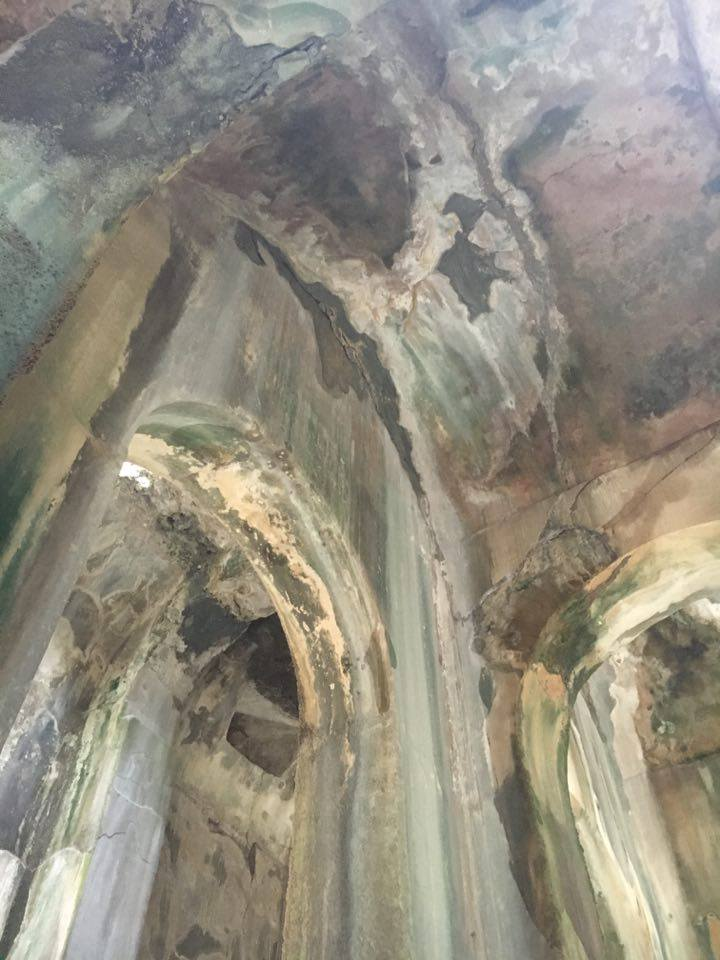
\includegraphics[width=\textwidth,height=12cm]{piscina_mirabilis.jpg}
  \caption{Microorganismal growth in the damp ancient cistern of Piscina Mirabilis in Bacoli.}
\end{figure*}

A case study of intertidal microorganisms and marine concrete in the United Kingdom by Coombes et al (2010) sheds light on the debate over the impact of microorganisms.  Over the course of eight months, marine concrete made of Portland concrete and crushed granite aggregate in Cornwall was covered by biochemical crusting and formed microcracks.  However, the locations of the crusting and microcracks were not correlated, suggesting that biological factors in that area do not contribute as much to concrete deterioration as might be thought.  The lack of correlation also frames the debate between those who believe that biological activity speeds up deterioration and those who believe that filmy microorganisms protect structures from further decay.  Although the study cannot be used to draw conclusions about Mediterranean concrete and biota because of the geographical distance between the two regions, it can inform the study of submerged concrete in the area that was the Roman empire.

	The most prominent microorganisms in the Bay of Naples provide some context for the kinds of potential deterioration in the region.  Along the coast of Italy, the most common fungal species include Corollospora maritima and Halosphaeriopsis mediosetigera (Cuomo et al 1988).  The outer walls of C. maritima are dark in color, meaning that it might warm the structure upon which it grows (Peng).  In the Underwater Archaeological Park of Baia, the most common algal species is Ostreobium quekettii.  Ricci et al (2013) found that Ichnoreticulina elegans, which is produced by O. quekettii, is responsible for many of the microfractures in calcareous artifacts.  Because algae also can damage concrete, the green algae in the Bay of Naples threatens all Roman remains and should be considered for new construction using any material.  
    
	In the Bay of Naples, existing ancient Roman concrete appears somewhat more resistant to biodeterioration than modern concrete.  Because the exposed sides of ancient Roman concrete are largely made from volcanic material, the ancient structures are better protected from bivalve boring than modern concrete.  The often calcareous aggregate used in modern concrete, in contrast, is more favorable to bivalve colonization.  Microorganisms grow similarly on both kinds of concrete, but the potential for heating from dark discoloration affects modern concrete more because it has a higher thermal conductivity than ancient Roman concrete.  From a biological perspective, pozzolana-based concrete made in the ancient Roman style is less susceptible to deterioration than is modern concrete,

\section*{Conclusion}

Ancient Roman concrete and modern concrete have been shown to respond differently to various physical and chemical stressors. Roman concrete's lower permeability, thermal conductivity, and chemical reactivity demonstrate its superior durability and longevity in the marine environment of the Bay of Naples. Assuming cost and availability are equal, Roman concrete would be an upgrade over modern concrete as a construction material for coastal communities.

Of course, availability and cost are not equal between RC and MC. While pozzolana is abundant in the Bay of Naples, its availability cannot rival the ubiquity of the ingredients for Portland cement and MC. Analyzing transport costs alone would crown MC as the more economical building material. Nevertheless, pozzolana components can be incorporated into MC recipes to bolster concrete durability in marine environments when necessary.

While RC shows impressive durability in the Bay of Naples, concrete degradation mechanisms still are relevant. Short of replacing ruins with replicas, there are few strategic decisions we can make to preserve the ancient ruins. Controlling the chemical content of the ocean or the atmospheric conditions is unfeasible, and removing species that contribute to concrete decay is unwise. Covering ruins in sedimentary layers is extremely effective, but interferes with visibility and tourism. Perhaps accepting degradation as a natural consequence of the passage of time is the best solution to this particular conservation issue.

\section*{References}
\begin{enumerate}

\item Agyekum Kofi, Joshua Ayarkwa, and Christian Koranteng. "Holistic Diagnosis of Rising Damp and Salt Attack in Two 
Residential Buildings in Kumasi, Ghana." Journal of Construction Engineering 2014 (2014): 1-13. Web. 2 July 
2016.

\item Banthia, N., O. E. Gjørv, and K. Sakai. Concrete under Severe Conditions: Environment and Loading: Proceedings of the 
Third International Conference on Concrete under Severe Conditions, CONSEC'01, Vancouver, BC, Canada, 
18-20 June 2001. Vancouver, B.C.:U of British Columbia, Dept. of Civil Engineering, 2001. Print.

\item Casoli E, Ricci S, Antonelli F, Perasso CS, Belluscio A, Ardizonne G. 2016. Impact and colonization dynamics of the bivalve Rocellaria dubia on limestone experimental panels in the submerged Roman city of Baiae (Naples, Italy). Intl. Biodeterioration and Biodegradation 108:9-15. 

\item Coombes MA, Naylor LA, Thompson RC, Roast SD, Gomez-Pujol L, Fairhurst RJ. 2011. Colonization and weathering of engineering materials by marine microorganisms: an SEM study. Earth Surface Processes and Landforms 36(5):582-593.

\item Cuomo V, Gareth Jones EB, Grasso S. 1988. Occurrence and distribution of marine fungi along the coast of the Mediterranean Sea. Prog. Oceanog. 21:189-200.

\item D. Campbell-Allen et al. The thermal conductivity of concrete. Magazine of Concrete Research

\item "Damage Caused By Sulfate Attack." St. Astier Blog. N.p., 30 Aug. 2012. Web. 02 July 2016.

\item Dias, B. B., M. B. Hart, C. W. Smart, and J. M. Hall-Spencer. "Modern Seawater Acidification: The Response of 
Foraminifera to High-CO2 Conditions in the Mediterranean Sea." Journal of the Geological Society167.5 (2010): 
843-46. Web.

\item Gaylarde C, Ribas Silva M, Warscheid Th. 2003. Microbial impact on building materials: an overview. Mat. Struct. 36(5):342-352.

\item Group, R. K. "Knowing Your Cements." Wonder of Cement (2014). 

\item Hao Yunhong, Yujiang Feng, and Jincheng Fan. "Experimental Study into Erosion Damage Mechanism of Concrete 
Materials in a Wind-blown Sand Environment." Construction and Building Materials 111 (2016): 662-70. Web.

\item Hasson, Dennis F., and C. R. Crowe. Materials for Marine Systems and Structures. Boston: Academic, 1988. Print.

\item International Organization for Standardization (ISO). "Building Materials and Products -- Hygrothermal properties -- Tabulated design values and procedures for determining declared and deigned thermal values"

\item Jaccarini V, Bannister WH, Micallef H. 1968. The pallial glands and rock boring in Lithophaga lithophaga (Lamellibranchia, Mytilidae). J. Zoo. 154:397-401.

\item Jackson D. Marie et al. 2013. Unlocking the Secrets of Al-tobermorite in Roman seawater concrete. 

\item Luchetta, A., C. Cantoni, and G. Catalano. "New Observations of CO 2 -induced Acidification in the Northern Adriatic Sea 
over the Last Quarter Century." Chemistry and Ecology 26.Sup1 (2010): 1-17. Web. 29 June 2016.

\item Morhange Ch, Bourcier M, Laborei J, Giallnella C, Goiran JP, Crimaco L, Vecchi L. 1999. New data on historical relative sea level movement in Pozzuoli, Phlaegrean Fields, Southern Italy. Phys. Chem. Earth (A) 24(4):349-354.

\item Morton B, Peharda M, Petric M. 2011. Functional morphology of Rocellaria dubia (Bivalvia: Gastrochaenidae) with new interpretations of crypt formation and adventitious tube construction, and a discussion of evolution within the family. Bio. Journal of the Linnean Society 104:786-804.

\item M Z Bessenouci et al. 2011. The apparent thermal conductivity of pozzolana concrete. 

\item Neville, Adam. "Chloride Attack of Reinforced Concrete: An Overview." Materials and 	Structures 28.2 (1995): 63-70.

\item Peng J. Corollospora maritima Werderm., 1922. Biota Taiwanica: Marine Fungi. http://marinefungi.taibif.tw/pages/1132.

\item Portland Cement Association. "Types and Causes of Concrete Deterioration". 

\item Ricci S, Perasso CS, Antonelli F, Petriaggi BD. 2015. Marine bivalves colonizing Roman artefacts recovered in the Gulf of Pozzuoli and in the Blue Grotto in Capri (Naples, Italy): Boring and nesting species. Intl. Biodeterioration and Biodegradation 98:89-100.

\item Ricci S, Pietrini AM, Bartolini M, Perasso CS. 2013. Role of the microboring marine organisms in the deterioration of archaeological submerged lapideous artifacts (Baia, Naples, Italy). Intl. Biodeterioration and Biodegration 82:199-206.

\item Winter, N. B. "Carbonation of Concrete." Understanding Cement. WHD, 2005. Web. 6 July 2016.

\end{enumerate}

\end{document}